% Options for packages loaded elsewhere
\PassOptionsToPackage{unicode}{hyperref}
\PassOptionsToPackage{hyphens}{url}
%
\documentclass[
]{article}
\usepackage{lmodern}
\usepackage{amssymb,amsmath}
\usepackage{ifxetex,ifluatex}
\ifnum 0\ifxetex 1\fi\ifluatex 1\fi=0 % if pdftex
  \usepackage[T1]{fontenc}
  \usepackage[utf8]{inputenc}
  \usepackage{textcomp} % provide euro and other symbols
\else % if luatex or xetex
  \usepackage{unicode-math}
  \defaultfontfeatures{Scale=MatchLowercase}
  \defaultfontfeatures[\rmfamily]{Ligatures=TeX,Scale=1}
\fi
% Use upquote if available, for straight quotes in verbatim environments
\IfFileExists{upquote.sty}{\usepackage{upquote}}{}
\IfFileExists{microtype.sty}{% use microtype if available
  \usepackage[]{microtype}
  \UseMicrotypeSet[protrusion]{basicmath} % disable protrusion for tt fonts
}{}
\makeatletter
\@ifundefined{KOMAClassName}{% if non-KOMA class
  \IfFileExists{parskip.sty}{%
    \usepackage{parskip}
  }{% else
    \setlength{\parindent}{0pt}
    \setlength{\parskip}{6pt plus 2pt minus 1pt}}
}{% if KOMA class
  \KOMAoptions{parskip=half}}
\makeatother
\usepackage{xcolor}
\IfFileExists{xurl.sty}{\usepackage{xurl}}{} % add URL line breaks if available
\IfFileExists{bookmark.sty}{\usepackage{bookmark}}{\usepackage{hyperref}}
\hypersetup{
  pdftitle={DM},
  pdfauthor={Vivien \& Louis},
  hidelinks,
  pdfcreator={LaTeX via pandoc}}
\urlstyle{same} % disable monospaced font for URLs
\usepackage[margin=1in]{geometry}
\usepackage{graphicx,grffile}
\makeatletter
\def\maxwidth{\ifdim\Gin@nat@width>\linewidth\linewidth\else\Gin@nat@width\fi}
\def\maxheight{\ifdim\Gin@nat@height>\textheight\textheight\else\Gin@nat@height\fi}
\makeatother
% Scale images if necessary, so that they will not overflow the page
% margins by default, and it is still possible to overwrite the defaults
% using explicit options in \includegraphics[width, height, ...]{}
\setkeys{Gin}{width=\maxwidth,height=\maxheight,keepaspectratio}
% Set default figure placement to htbp
\makeatletter
\def\fps@figure{htbp}
\makeatother
\setlength{\emergencystretch}{3em} % prevent overfull lines
\providecommand{\tightlist}{%
  \setlength{\itemsep}{0pt}\setlength{\parskip}{0pt}}
\setcounter{secnumdepth}{-\maxdimen} % remove section numbering

\title{DM}
\author{Vivien \& Louis}
\date{01/03/2021}

\begin{document}
\maketitle

\hypertarget{question-1}{%
\section{Question 1}\label{question-1}}

Le meilleur estimateur de \({f}(x)\) au sens de l'erreur quadratique
moyenne intégrée est l'estimateur de Parzen-Rosenblatt
\(\hat{f}(x) = \frac{1}{nh_{cv}}\sum_{j=1}^{n}K(\frac{x-X_{j}}{h_{cv}})\)
ou K est un noyau choisi et \(h_{cv}\) petit obtenue par validation
croisé \emph{leave-one-out}.

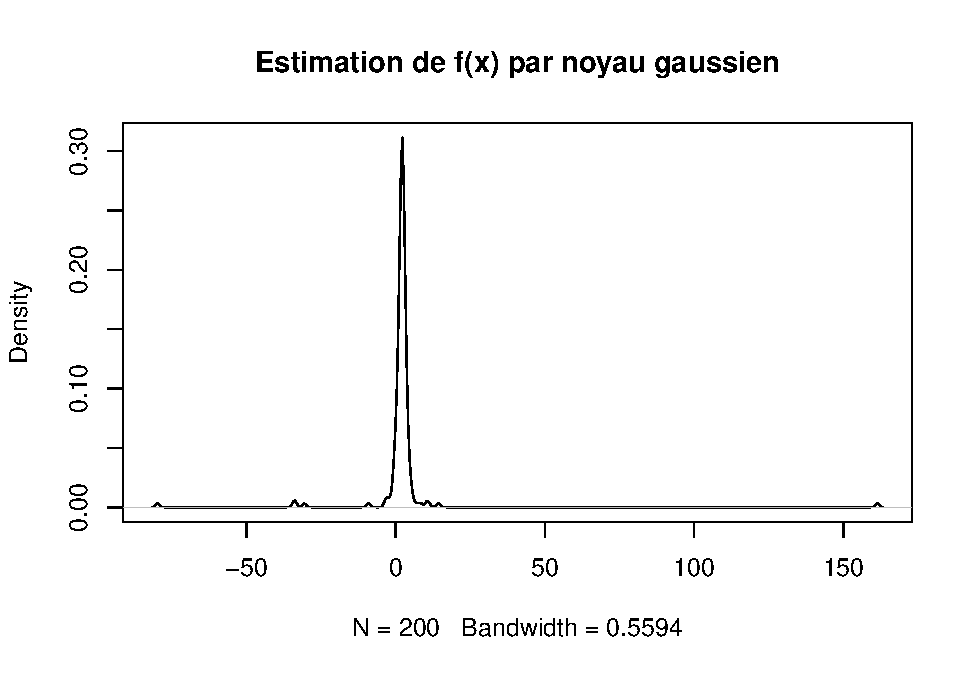
\includegraphics{DM_files/figure-latex/unnamed-chunk-2-1.pdf}

\hypertarget{question-2}{%
\section{Question 2}\label{question-2}}

\begin{itemize}
\tightlist
\item
  Puisque l'on estime une loi de densité (semblant continue de par les
  nombreux chiffres après la virgule des observations) on souhaite que
  notre estimation ait les bonnes propriétés associées aux lois de
  densité. Ainsi il vient naturellement que le noyau \(K\) doit être une
  densité de probabilité, lisse, continue et différentiable. Par défaut
  et sans information supplémentaire j'ai décidé de retenir le noyau
  gaussien. De plus, en faisant exception des valeurs extrêmes de notre
  echantillon, la partie centrale de la distribution de notre
  echantillon semble suivre une loi normale.
\end{itemize}

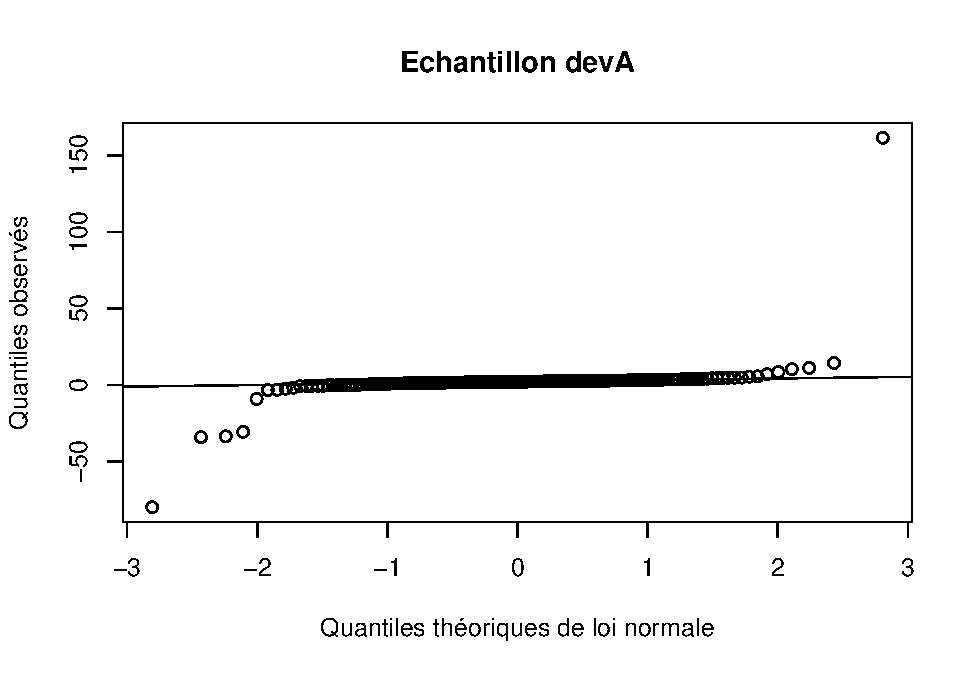
\includegraphics{DM_files/figure-latex/unnamed-chunk-3-1.pdf}

\begin{itemize}
\tightlist
\item
  Le choix de la fenêtre \(h\) est réalisé par validation croisée
  \emph{leave-one-out} puisque
  \(h_{cv} = arg min_{h}[\int \hat{f}^2_{n}(x)dx - \frac{2}{n}\sum_{i=1}^{n}\hat{f}_{-i}(X_{i})]\).\\
  \(h_{cv}\) est alors égal à 0.5593725.
\end{itemize}

\hypertarget{question-3}{%
\section{Question 3}\label{question-3}}

\(f(x)\) est une loi symétrique par rapport à \(\theta_{0}\). Par
conséquent, on peut estimer graphiquement \(\theta_{0}\) par l'abscisse
du point de maximum de la courbe. \emph{i.e.}

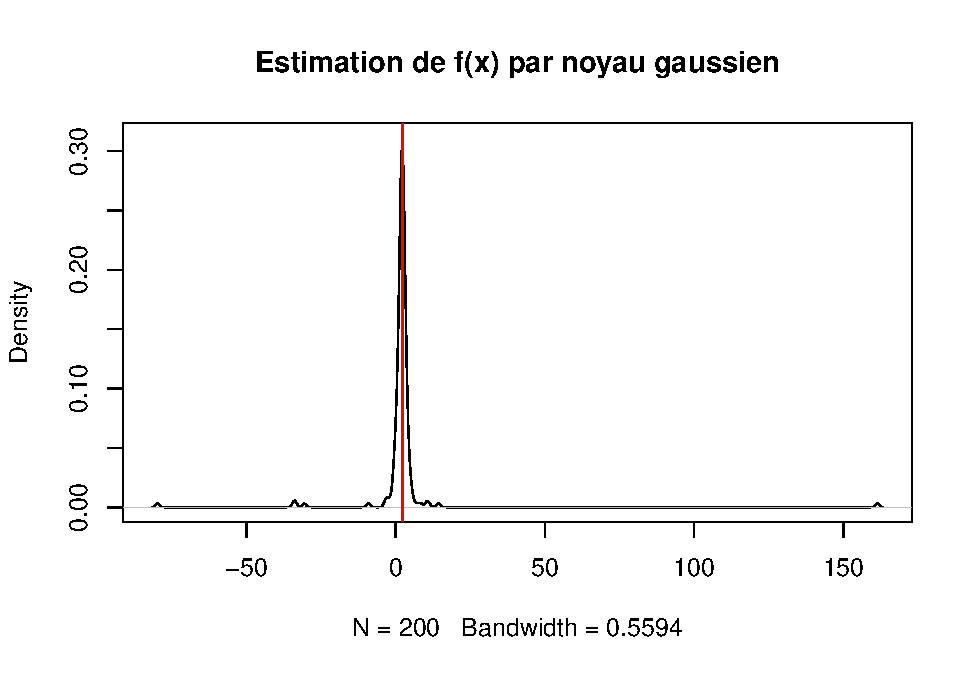
\includegraphics{DM_files/figure-latex/unnamed-chunk-4-1.pdf}

On approxime alors \(\theta_{0}\) par \(\theta_{0}^{approx} =\)
2.2656625.

\hypertarget{question-4}{%
\section{Question 4}\label{question-4}}

On peut faire mieux que ces approximations :

On choisit le noyau gaussien :
\(K(x) = \frac{1}{\sqrt{2\pi}}exp(-x^2/2)\)\\
notre fonction de densité est estimée par l'estimateur de
Nadaraya-Watson :
\(\hat{f}_{n}(x)=\frac{1}{nh}\sum_{i=1}^{n}K(\frac{x-X_i}{h})\)\\
la largeur de fenêtre obtenue par validation croisée : \(h_{cv}\) =
0.5593725

Or :\\
\(\tilde{\theta} = argmax_{\theta} \sum^{n}_{i=1}ln\hat{f}_{n}(2\theta-X_i)\)\\
\(\tilde{\theta} = argmax_{\theta}\sum_{i=1}^{n}ln[\frac{1}{nh}\sum_{j=1}^{n}K(\frac{2\theta-X_i-X_j}{h})]\)\\
\(\tilde{\theta} = argmax_{\theta}\sum_{i=1}^{n}ln\sum_{j=1}^{n}K(\frac{2\theta-X_i-X_j}{h})\)

On dérive la fonction dans le argmax par rapport à \(\theta\) afin de la
maximiser :

\(g^{'}(\theta)= \sum^{n}_{i=1}\sum^{n}_{j=1}\frac{K^{'}(\frac{2\theta-X_i-X_j}{h})}{K(\frac{2\theta-X_i-X_j}{h})}\)

\(g^{'}(\theta)= \sum^{n}_{i=1}\sum^{n}_{j=1}\frac{(\frac{-2\theta}{h^2} + \frac{X_i}{h^2} + \frac{X_j}{h^2})exp(-(\frac{2\theta - X_i -X_j}{h})^2/2)}{exp(-(\frac{2\theta - X_i -X_j}{h})^2/2)}\)

\(g^{'}(\theta)= \sum^{n}_{i=1}\sum^{n}_{j=1}(2\theta + X_i + X_j)\)

\(g^{'}(\theta)= 0\)

équivaut à :

\(2n^{2}\theta - n^{2}\bar{X_n} - n^{2}\bar{X_n}=0\)

\(\tilde{\theta} = \bar{X_n}\)

Ainsi en prenant le noyau gaussien et un paramètre de lissage optimal
par validation croisée on trouve que l'estimateur asymptotiquement
efficace pour \(\theta\) est \(\bar{X_n}=\) 2.0501181\\
Or, \(E[\bar{X_n}] = \frac{1}{n}\sum_{i=1}^{n}E[X1]\) car les \(X_i\)
sont indépendants deux à deux, qu'ils sont issus de la même loi de
densité \(f(x)\) et que \(X_i\) semble converger dans \(L^1\). Ainsi par
la loi des grands nombres : \(\tilde{\theta}\) converge vers la vraie
valeurs de \(\theta\) asymptotiquement.

\hypertarget{partie-b}{%
\section{Partie B}\label{partie-b}}

\hypertarget{question-1-1}{%
\section{Question 1}\label{question-1-1}}

Sachant que les données observées sont issues d'une régression, que nos
valeurs manquantes sont en fait des réponses et que l'hypothèse des
observations MAR est satisfaite on a :

\(Y=m(X)+\epsilon\) , \(E( \epsilon |X)=0\) et
\(Y {\perp \!\!\! \perp}D,X\).

On souhaite estimer l'esperance de Y avec l'estimateur de
Nadaraya-Watson:
\(\hat r(u)=\frac{\sum Z_iK(\frac{u-U_i}{h})}{\sum K(\frac{u-U_i}{h})}\)
avec K le noyau et h la fenêtre.

On sait que \(P(X)=P(D=1|X)=E(D|X)\) donc on a :

\(m(X)=E(Y|X)=\frac {E(DY|X)}{E(D|X)}\). On applique l'estimateur de
Nadaraya-Watson sur E(DY\textbar X) et E(D\textbar X) et on obtient

\(E(DY|X)=\frac{\sum D_i Y_i K(\frac {x-X_i}{h})}{\sum K(\frac {x-X_i}{h})}\)
et
\(E(D|X)=\hat p(X)=\frac{\sum D_i K(\frac {x-X_i}{h})}{\sum K(\frac {x-X_i}{h})}\)

ce qui nous donne l'estimateur \(\hat m_n\) de m en simplifiant:

\(\hat m_n(x)=\frac{\sum D_i Y_i K(\frac {x-X_i}{h})}{\sum D_iK(\frac {x-X_i}{h})}\)

On cherche à écrire un programme permettant de calculer l'estimateur
\(\hat \alpha_n\) de \(\alpha_0 =E(Y)\). On a calculé deux estimateurs
de \(\alpha_0\) tels que \(\hat \alpha_{n,1}= \sum \hat m(X_i)/n\) et
\(\hat \alpha_{n,2}= \frac {1}{n}\sum [\frac{D_i Y_i}{\hat p(X_i)}+(1-\frac {D_i}{\hat p(X_i)})\hat m(X_i)]\)

Pour ceci, nous avons construit les fonctions retournant respectivement
\(\hat p\) et \(\hat m\) pour un certain x et un paramètre de lissage h
en appliquant la contrainte D=1.Nous avons choisi tout d'abord h=5
d'après un critère graphique mais nous calculerons sa valeur optimale
par une validation croisée ultérieurement.

Puis, il a fallu appliquer ces fonctions à l'ensemble des \(X_i\) avec
la fonction sapply() retournant ainsi un vecteur de valeurs. Il suffit
ensuite de construire les estimateurs \(\hat\alpha_{n,1}\) et
\(\hat \alpha_{n,2}\) avec ces valeurs

Avec h=5 on obtient \(\hat \alpha_{n,1}\) =0.9173743 et
\(\hat \alpha_{n,2}\)= 0.9173858

Nous calculons ensuite le paramètre de lissage h optimal par validation
croisée. Puisque \(\hat p\) et \(\hat m\) sont des estimateurs de
regression différents, il faut trouver un h par validation croisée pour
chacun d'entre eux.

Calculons tout d'abord l'estimateur \(h_{p_{CV}}\) le paramètre de
lissage de \(\hat p\). On fait une validation croisée en leave-1-out en
prenant:

\(h_{p_{CV}}=\arg\min_h \frac{1}{n}\sum[D_i-\hat p_{n,h}^{(-i)}(X_i)]^2\)

avec
\(\hat p_{n,h}^{(-i)}=\frac{\sum\limits_{j\neq i}^n D_j K(.)}{\sum \limits_{j\neq i}^n K(.)}\)

On construit un premier algorythme pour déterminer les
\(\hat p_{n,h}^{(-i)}\) avec une fonction prenant en argument une
observation x, un paramètre de lissage h qui variera à l'avenir et un
paramètre k permettant de retirer l'observation i. Cette fonction
retourne la valeur de \(\hat p_{n,h}^{(-i)}\) pour un \(x_i\) fixé en
vérifiant si \(Y_i\) est observé.

Une deuxième fonction prenant en argument h pour faire varier le
paramètre de lissage et retournant la valeur \(h_{p_{CV}}\) applique la
fonction ci-dessus en différençiant les 200 \(Y_i\) observés ou non.

\begin{verbatim}
## [1] 1.069
\end{verbatim}

En appliquant à la dernière fonction plusieurs séquences de h
différents, on essaye de determiner une approximation de h optimale
c'est à dire la valeur de h pour laquelle \(h_{p_{CV}}\) est
\(\arg\min_{h} \frac{1}{n}\sum[D_i- \hat p_{n,h}^{(-i)}(X_i)]^2\) . On
trouve donc pour \(h_{p_{CV}}\) la valeur 1.069

Maintenant qu'on a trouvé le \(h_{p_{CV}}\) par validation croisée pour
\(\hat p\) on va faire une validation croisée pour \(\hat m\).
l'estimation de h pour l'estimateur \(\hat m\) par la validation croisée
qui va

vérifier
\(h_{CV}=\arg\min_{h} \frac{1}{n}\sum[\frac{D_iY_i}{\hat p_{n,h}^{(-i)}}- \hat m_{n,h}^{(-i)}(X_i)]^2\)

avec
\(\hat m_{n,h}^{(-i)}=\frac{\sum\limits_{j\neq i}^n D_jY_j K(.)}{\sum \limits_{j\neq i}^n D_jK(.)}\)

Pour construire un algorithme permettant de determiner une approximation
de h, il est néccessaire de construire \(\hat m_{n,h}^{(-i)}\)

Dans la même logique que pour \(h_{p_{CV}}\), on construit un premier
algorythme pour déterminer les \(\hat m_{n,h}^{(-i)}\) avec une fonction
prenant en argument une observation x, un paramètre de lissage h qui
variera à l'avenir et un paramètre k permettant de retirer l'observation
i. Cette fonction retourne la valeur de \(\hat m_{n,h}^{(-i)}(X)\)

Une deuxième fonction prenant en argument h pour faire varier le
paramètre de lissage et retournant la valeur \(h_{CV}\) applique la
fonction ci-dessus en différençiant les 200 \(Y_i\) observés ou non.
Dans cette fonction, on applique la valeur optimale de \(h_{p_{CV}}\)
pour la valeur de \(\hat p_{n,h}^{(-i)}\) calculée prédédemment.

\begin{verbatim}
## [1] 0.6
\end{verbatim}

En appliquant à la dernière fonction plusieurs séquences de h
différents, on essaye de determiner une approximation de h optimale
c'est à dire la valeur de h pour laquelle \(h_{CV}\) est minimal. On
trouve donc pour \(h_{CV}\) la valeur 0.6

On remplace ainsi ensuite la valeur h=5 par h=1.069 pour \(\hat p\) et
h=0.6 pour \(\hat m\) dans les fonctions permettant de calculer ces
estimateurs

On obtient \(\hat \alpha_{n,1}\) =0.8078243 et \(\hat \alpha_{n,2}\)=
0.9011848 ce qui est proche de la moyenne empirique. Par résultat du
cours \(\hat \alpha_{n,1}\) et \(\hat \alpha_{n,2}\) sont des
estimateurs consistants et asyptotiquement efficaces de
\(\alpha_o= E(Y)\). On aurait aussi pu appliquer la loi des grands
nombres pour le prouver

\hypertarget{question-2-1}{%
\section{Question 2}\label{question-2-1}}

Pour le choix des paramètres de lissage, nous avons choisi de les
determiner par validation croisée leave-one-out car cette méthode
minimise les erreurs de prédiction. Quant à la méthode, nous avons
appliqué l'estimateur de NW à un jeu de données avec valeurs manquantes
en prenant un noyau gaussien. Le choix du noyau importe peu, seul le
choix du paramètre de lissage permet de réaliser un arbitrage
Biais-variance.

\end{document}
